\chapter{Analysis}\label{analysis}
In this chapter several attacks as listed in Section~\ref{attack-models} will be shown. The methods and

\section{Holiday and Sick Leave Detection}

The information about anomalies in the regular work pattern can be a valuable information for several parties.
Usually only few parties people know about the holiday or sick leave times of a person.
To know if a persons tends to become sick often or for long times is a dangerous intrusion into a persons privacy.
For instance this could be abused by head hunters or personnel managers to cull possible employees with too high sick leave rates and thereby reduce the job prospects of the target.

For employees this might convenient to detect anomalies in the productivity of an employee.
In case an employee doesn't commit on a regular basis for several days, this behaviour would be instantly visible with this method.

Another attack vector could be to look at the correlation of missing time between several employees.
This attack could even be performed by an outsider, if the employees of a company are known.
The information gained by this attack could be quite delicate, as they could reveal relationships between employees.
This attack is heavily inspired by an article about data mining articles from the popular German weekly magazine \emph{Der Spiegel} written by the David Kriesel~\cite{article:spiegel-mining}.


\subsection{Implementation}

The requirements for this algorithm is the detection of a regular work pattern for a given interval.
It must have the ability to adjust to a changing work pattern, but at the same time has to be capable of detecting anomalies in this pattern.
If the attacker wants to look at multiple people, some kind of measure for similarity in the missing time patterns has to exist.

The input for this analysis is the intersection between all commits from the considered repositories and all commits from the considered contributors.
The commits' meta data used for this analysis are time stamps as well as additions and deletions in lines of code.

\begin{figure}[H]
    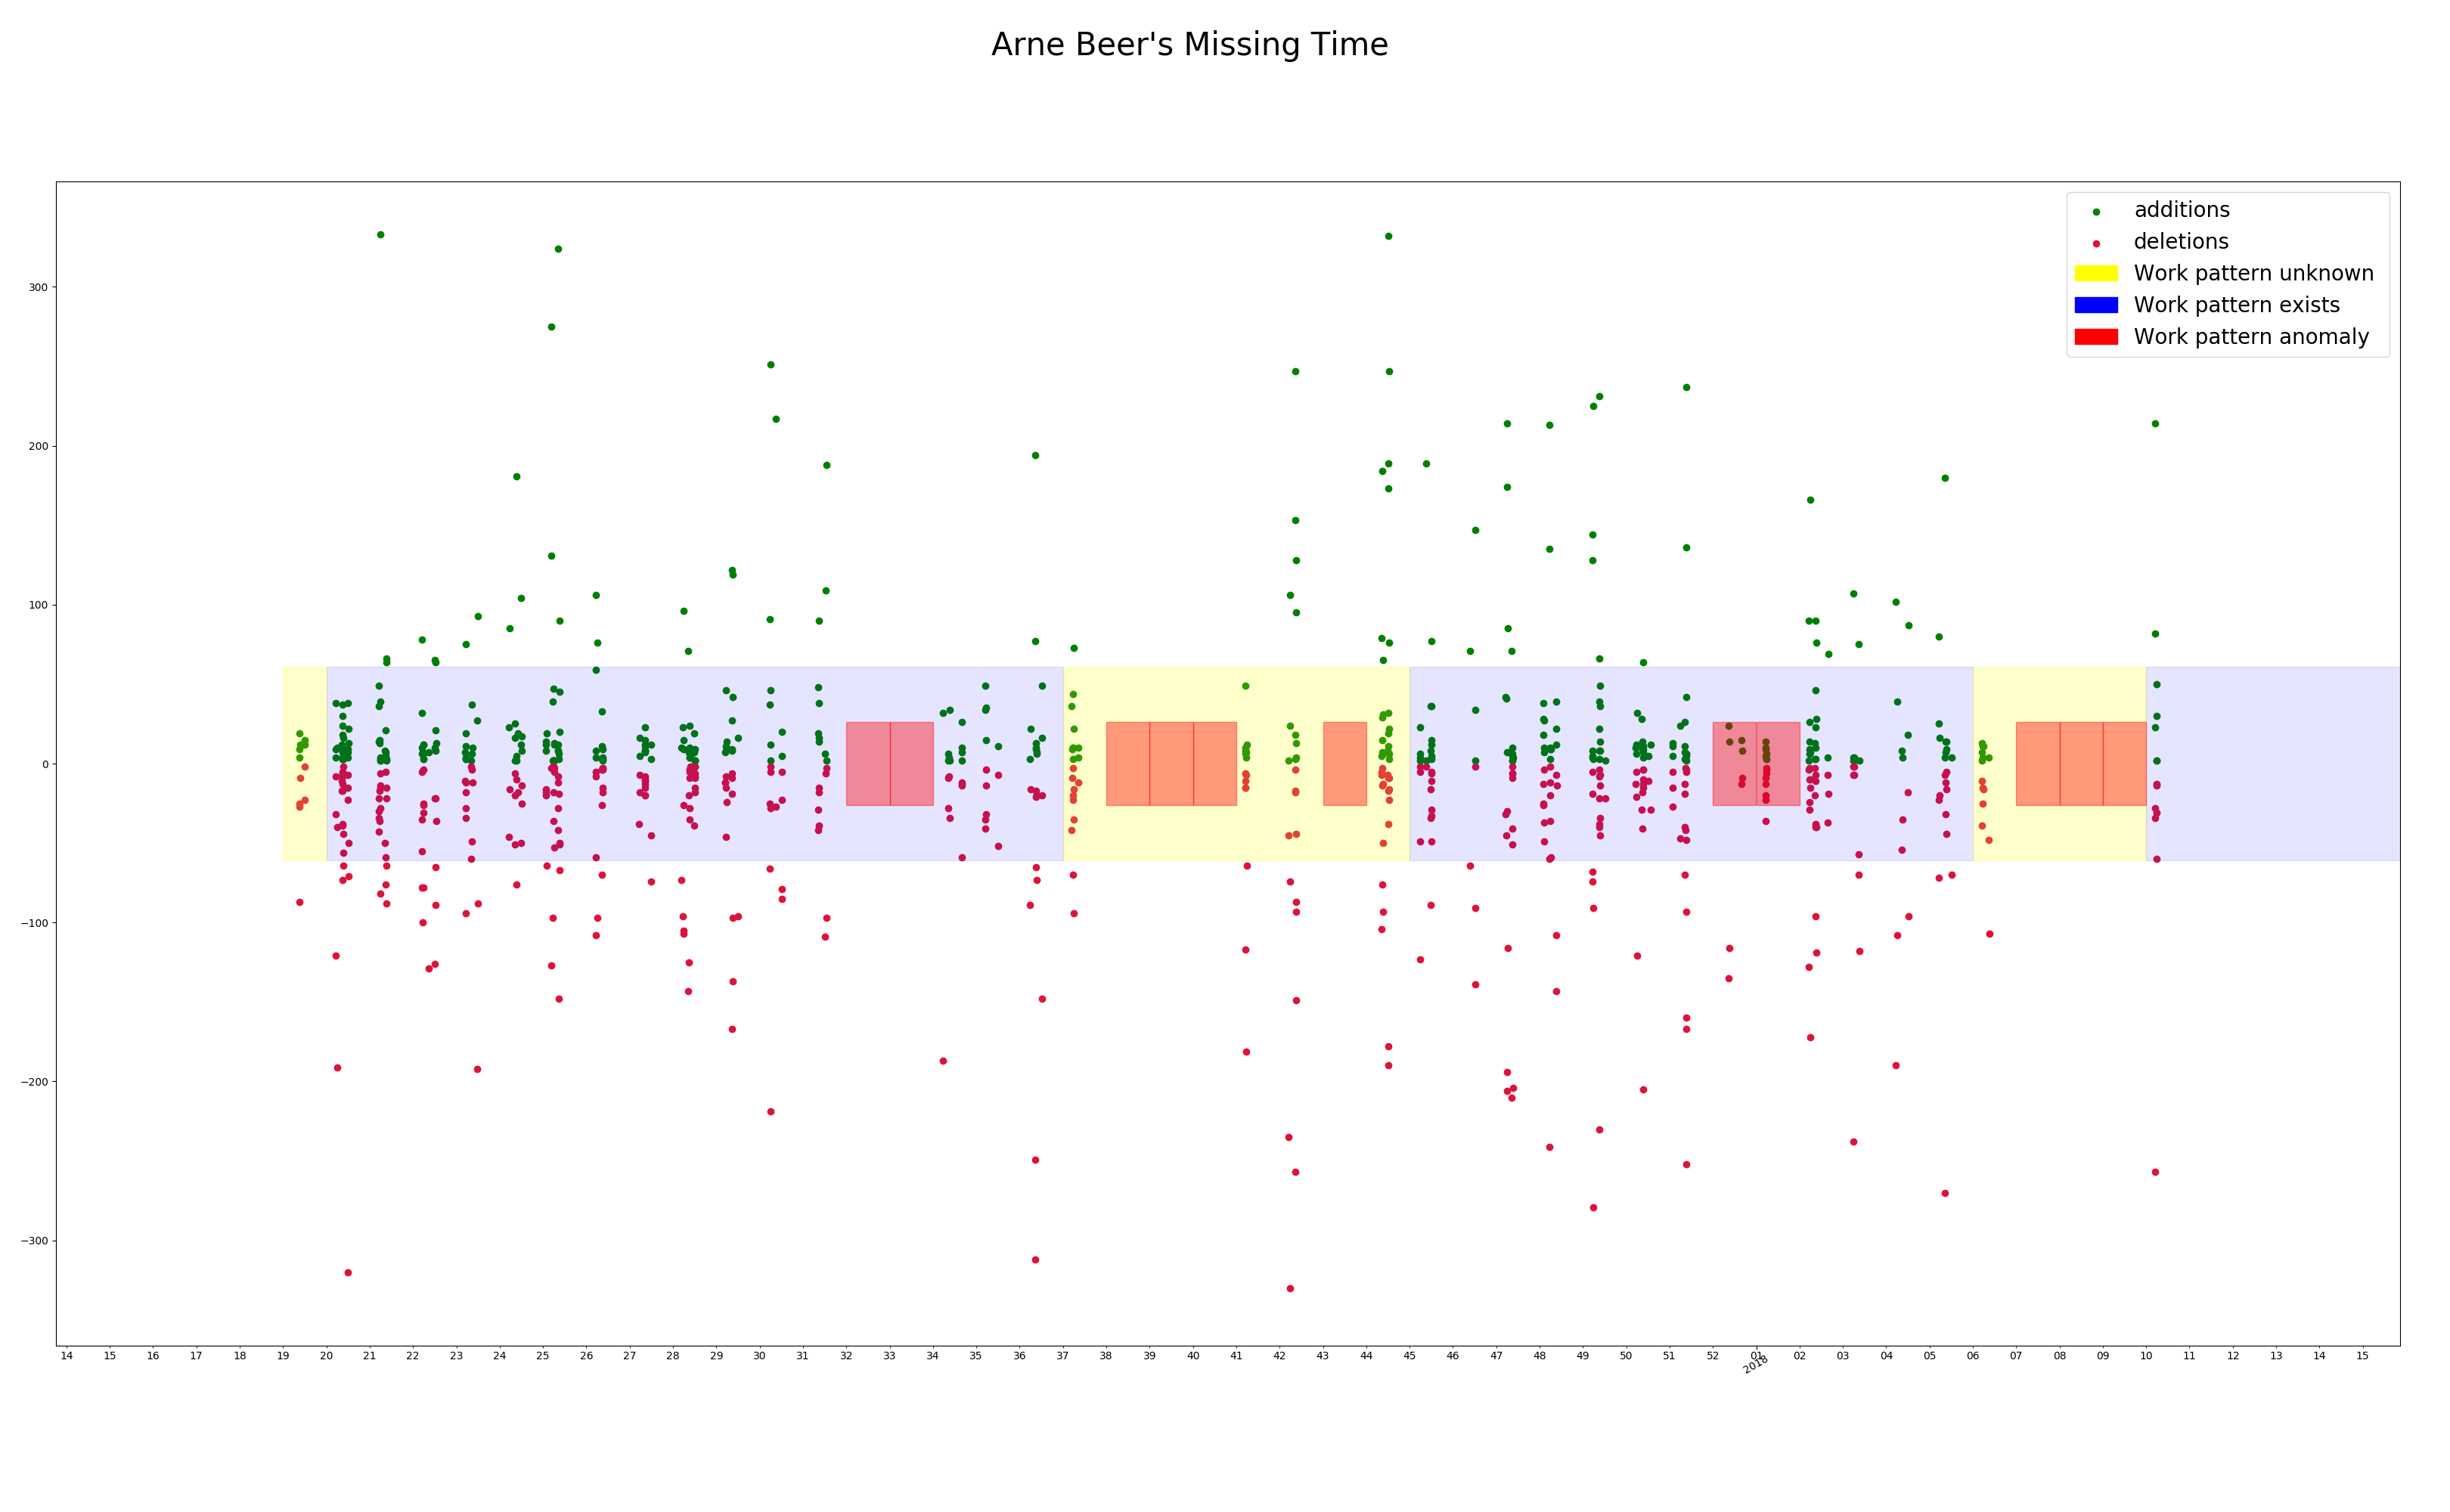
\includegraphics[scale=0.21]{./graphs/analysis/work-time-analysis}
    \centering
    \caption{The work time analysis of the author.}\label{fig:missing-time}
\end{figure}

The analysis of the data is a chronological scan of all commits for specific user.
Before performing the actual analysis, the data is converted into a usable format representing the week days.
The converted data format represents the amount of commits for each day in the last year.
It is really difficult to measure productivity in lines of code committed or in the amount of commits made by a person, as they don not necessarily display the amount of work that have been put into those commits.
As a result I decided, that a day counts as a work day as long as at least single commit has been made during the day.

\begin{minted}{python}
    prototype = None
    while len(weeks) > 0:
        week = weeks.pop
        if not prototype:
            # See if there is a prototype in the next few weeks.
            prototype = find_prototype(week, weeks)

            # Check if this specific week is a anomaly
            check_anomaly(prototype, week)

            continue


        prototype_exists = prototype_in_next_weeks(weeks)
        if not prototype_exists:
            # We couldn't find the prototype in the next few rows
            # Try to find a new prototype
            prototype = find_prototype(week, weeks)

        check_anomaly(prototype, week)
\end{minted}

The algorithm looks at every week of the past year.
At the beginning of the algorithm it tries to find a new \emph{prototype}.
A prototype is a representative week work pattern, which resembles at least four weeks in the next six weeks.

If a prototype is found, we are capable of identifying anomalies that deviate from this pattern.
For each following week is checked, if it is considerably different from the prototype and if there exists an identical week pattern in the near future.
If there is no identical pattern in the near future, the current work pattern ends and a new prototype needs to be found.

In case no prototype exists, anomalies cannot be easily identify and will only be marked as such, in case of obvious anomalies like weeks completely without commits.
Each week will be inspected and a new prototype tried to be found.
